\documentclass{elsarticle}

\usepackage{amsmath}
\usepackage{graphics}
\usepackage{graphicx}
\usepackage{subfigure}
\usepackage{color}
\usepackage{xspace}
\usepackage{url}
\usepackage[utf8]{inputenc}

% reviews
\newcommand{\todo}[1]        {\textcolor{red}{[TODO] #1}}
\newcommand{\keoma}[1]       {\textcolor{blue}{[Keoma] #1}}
\newcommand{\remy}[1]        {\textcolor{blue}{[Remy] #1}}
\newcommand{\xavi}[1]        {\textcolor{blue}{[Xavi] #1}}
\newcommand{\thomas}[1]      {\textcolor{blue}{[Thomas] #1}}

 % lorem
\newcommand{\lorem}          {\textcolor{green}{Lorem ipsum dolor sit amet, consectetur adipisicing elit, sed do eiusmod tempor incididunt ut labore et dolore magna aliqua. Ut enim ad minim veniam, quis nostrud exercitation ullamco laboris nisi ut aliquip ex ea commodo consequat. Duis aute irure dolor in reprehenderit in voluptate velit esse cillum dolore eu fugiat nulla pariatur. Excepteur sint occaecat cupidatat non proident, sunt in culpa qui officia deserunt mollit anim id est laborum.}}

% shortcuts
\newcommand{\smip}                {SmartMesh~IP\xspace}
\newcommand{\HRNEIGHBORS}         {{\tt HR\_NEIGHBORS}\xspace}
\newcommand{\HRDISCOVERED}        {{\tt HR\_DISCOVERED}\xspace}
\newcommand{\HRDEVICE}            {{\tt HR\_DEVICE}\xspace}
\newcommand{\pathcreate}          {{\tt path\_create}\xspace}
\newcommand{\pathdelete}          {{\tt path\_delete}\xspace}
\newcommand{\motecreate}          {{\tt mote\_create}\xspace}
\newcommand{\moteId}              {{\tt moteId}\xspace}
\newcommand{\NUMHRNEIGHBORS}      {140,897\xspace}
\newcommand{\NUMSTATS}            {369,276\xspace}

\graphicspath{{figures/}}

\begin{document}
	
\begin{frontmatter}
	
\title{(Not so) Intuitive Results from a Smart Agriculture\\Low-Power Wireless Mesh Deployment}

\author[inria]{Keoma~Brun-Laguna}
	\ead{keoma.brun@inria.fr}
\author[inria]{R\'emy~L\'eone}
    \ead{remy.leone@inria.fr}
\author[uoc]{Xavier~Vilajosana}
    \ead{xvilajosana@uoc.edu}
\author[inria]{Thomas~Watteyne}
    \ead{thomas.watteyne@inria.fr}

\address[inria]{Inria, EVA team, Paris, France}
\address[uoc]{Univ. Oberta de Catalunya, Barcelona, Catalonia, Spain}

\end{frontmatter}

\begin{abstract}
\lorem
\end{abstract}

%==============================================================================
\section{Introduction}
\label{sec:intro}

% the problem

\lorem

% the PEACH project

\lorem

%======== front-page figure, do not move
\begin{figure}
    \centering
    
\includegraphics[width=\columnwidth]{fake}
    \caption{The wireless motes deployed in the peach orchard in Mendoza, Argentina.}
    \label{fig:orchard}
\end{figure}

% the architecture

\lorem

\begin{figure*}
    \centering
    
\includegraphics[width=\textwidth]{fake}
    \caption{Areal view of the sensor network deployed in the orchard near Mendoza, Argentina.}
    \label{fig:map}
\end{figure*}

% the deployment

\lorem

% hardware
\lorem

% technology

\lorem

% the data

\lorem

% the goal of this paper

\lorem

% paper organisation

\lorem

%==============================================================================
\section{Statistics Collected}
\label{sec:collected}

% environment

\lorem

% events and HR

\lorem

% number received and remainder

\lorem

% analysis

\lorem

%==============================================================================
\section{Intuitive Results}
\label{sec:intuitive}

\lorem

%------------------------------------------------------------------------------
\subsection{RSSI vs. Distance}
\label{sec:rssi_distance}

\lorem

\begin{figure}[h]
    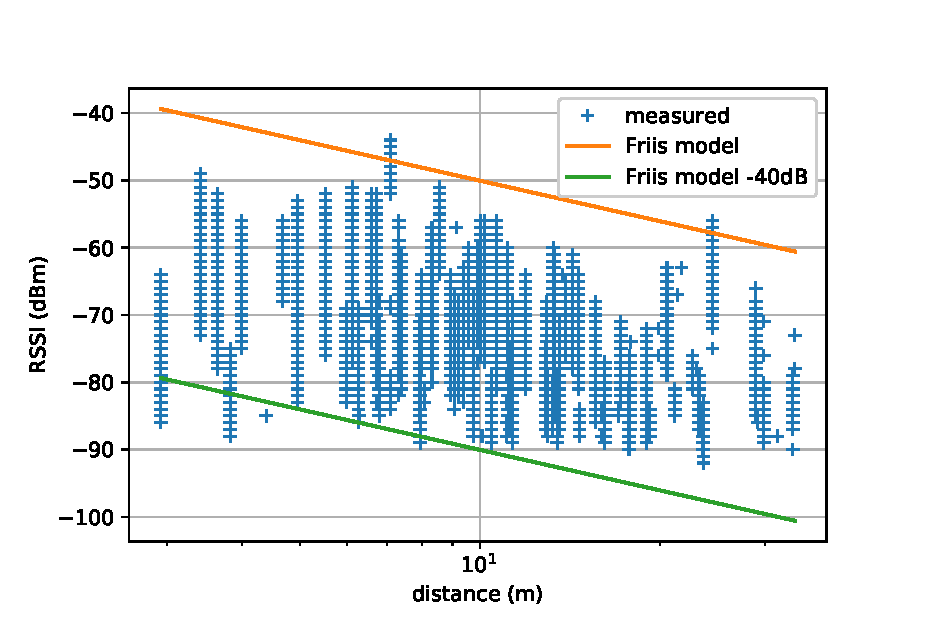
\includegraphics[width=0.5\columnwidth]{pister_hack.eps}
    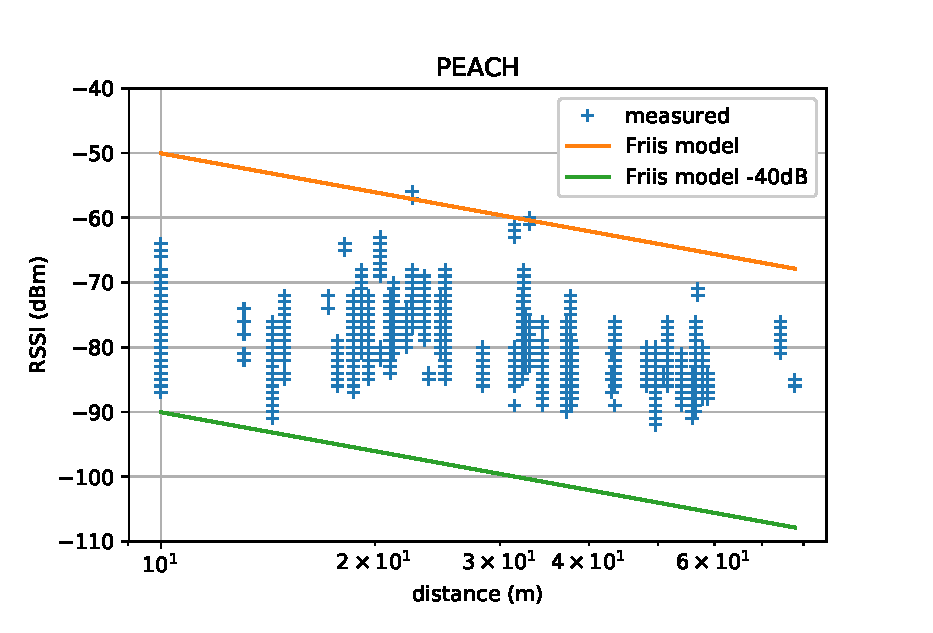
\includegraphics[width=0.5\columnwidth]{pister_hack_peach.eps}
    \caption{RSSI measurements are roughly located between the Friis model and the Friis model shifted by $-$40~dB.}
    \label{fig:pister_hack}
\end{figure}

%------------------------------------------------------------------------------
\subsection{Wireless Waterfall}
\label{sec:waterfall}

% sample presentation

\lorem

% plot

\begin{figure}
    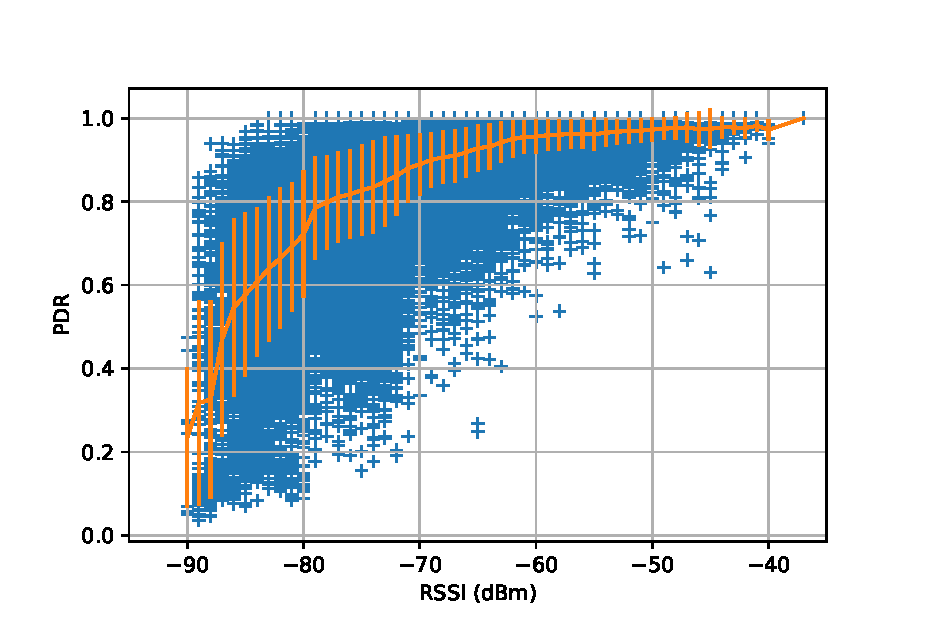
\includegraphics[width=0.5\columnwidth]{waterfall.eps}
    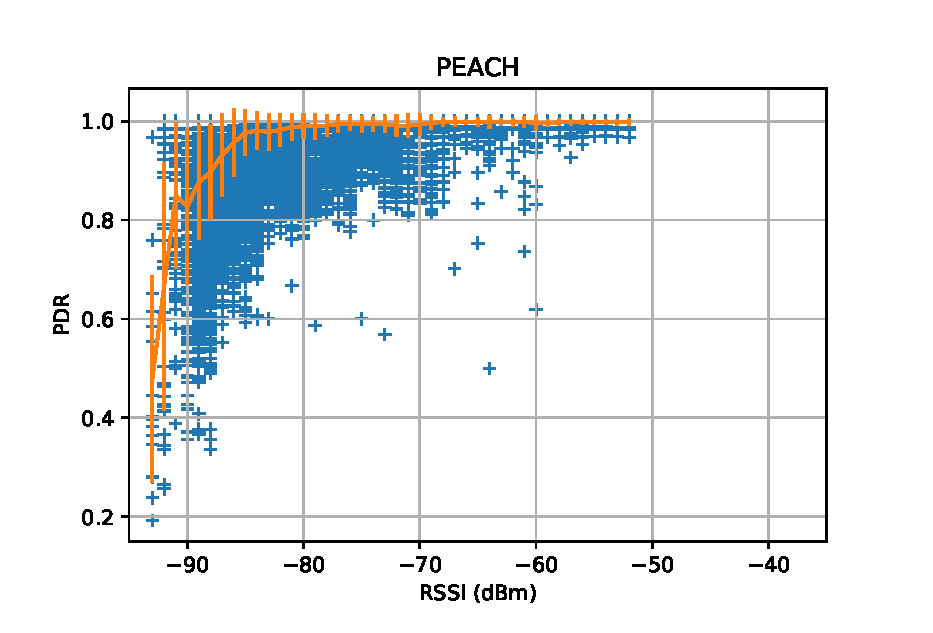
\includegraphics[width=0.5\columnwidth]{waterfall_peach.eps}  
    \caption{
        The PDR/RSSI ``waterfall'' plot.
    }
    \label{fig:waterfall}
\end{figure}

\lorem

% interferences

\lorem

%------------------------------------------------------------------------------
\subsection{End-to-End Reliability}
\label{sec:net_reliability}

% steady state results

\lorem

\begin{table}
    \begin{tabular}{|l|l|}
        \hline
        reliability & XX\% (Arrived/Lost:   /)\\ \hline
        average PDR & XX\% (Transmit/Fails: /)\\ \hline
        latency     & XXXX~msec\\
        \hline
    \end{tabular}
    \caption{The overall network performance in the 15-25 July 2016 period.}
    \label{tab:net_stats}
\end{table}

\lorem

%------------------------------------------------------------------------------
\subsection{Network Lifetime}
\label{sec:lifetime}

% description

\lorem

% results

\lorem

\begin{table}
    \begin{tabular}{|c|c|r|}
        \hline
        MAC address    & charge consumed           &   lifetime \\
        \hline
        \tt{30-60-ef}  & 227,847~C (2.2\% battery) & 10.8~years \\
        \tt{38-0f-66}  & 252,356~C (2.5\% battery) &  9.8~years \\
        \tt{3f-f8-20}  & 291,312~C (2.9\% battery) &  8.4~years \\
        \tt{3f-fe-87}  & 392,606~C (3.9\% battery) &  6.3~years \\
        \tt{3f-fe-88}  & 458,459~C (4.5\% battery) &  5.3~years \\
        \tt{58-32-36}  & 327,634~C (3.2\% battery) &  7.5~years \\
        \tt{60-01-f8}  & 252,454~C (2.5\% battery) &  9.8~years \\
        \tt{60-02-1b}  & 222,253~C (2.2\% battery) & 10.1~years \\
        \tt{60-02-4b}  & 146,068~C (1.4\% battery) & 16.8~years \\
        \tt{60-03-82}  & 494,841~C (4.9\% battery) &  5.0~years \\
        \tt{60-05-5f}  & 274,502~C (2.7\% battery) &  9.0~years \\
        \tt{60-05-69}  & 437,136~C (4.3\% battery) &  5.7~years \\
        \tt{60-05-78}  & 304,145~C (3.0\% battery) &  8.1~years \\
        \tt{60-05-ab}  & 284,764~C (2.8\% battery) &  8.7~years \\
        \tt{60-06-27}  & 321,879~C (3.2\% battery) &  7.7~years \\
        \tt{60-08-d5}  & 263,120~C (2.6\% battery) &  9.3~years \\
        \hline
    \end{tabular}
    \caption{Per-node power consumption and associated expected lifetime when powered by a pair of AA batteries.}
    \label{tab:stats_charge}
\end{table}

%==============================================================================
\section{Not so Intuitive Results}
\label{sec:notsointuitive}

\lorem

%------------------------------------------------------------------------------
\subsection{Link (A)Symmetry}
\label{sec:symmetry}

% what is reported

\lorem

% what is asymmetry

\lorem

% what we measure

\lorem
\begin{figure}
    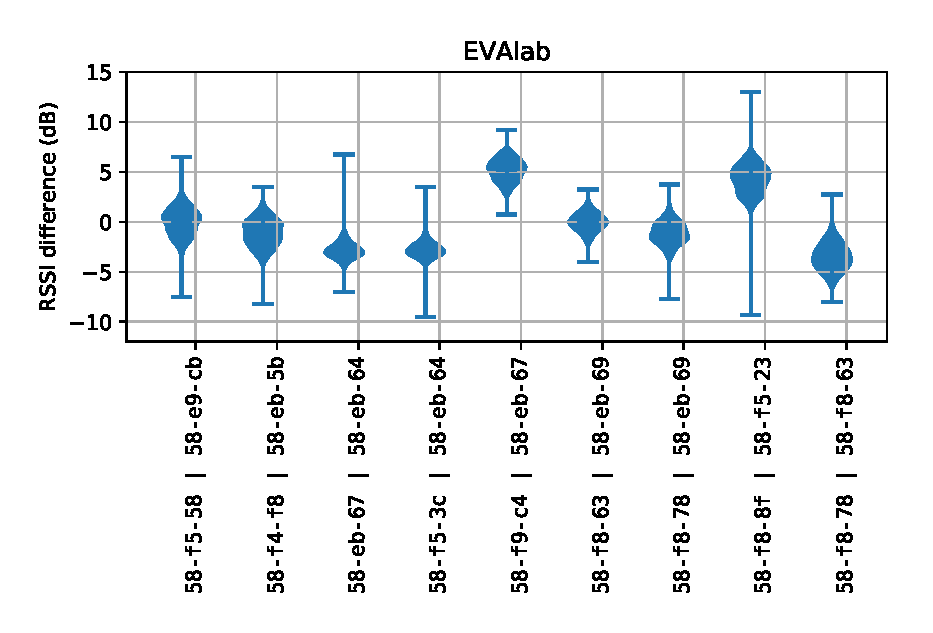
\includegraphics[width=0.5\columnwidth]{asymmetry.eps}
    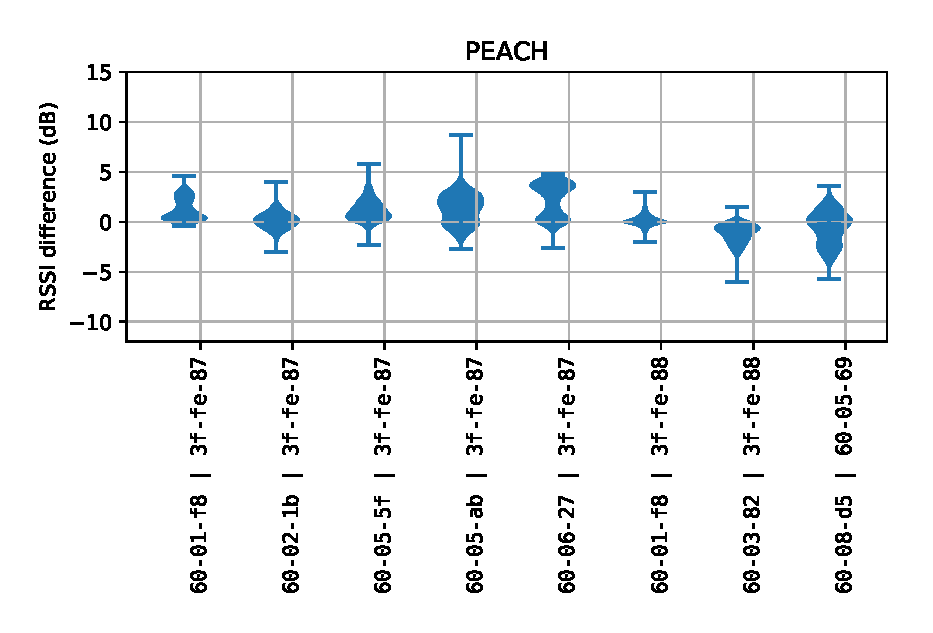
\includegraphics[width=0.5\columnwidth]{asymmetry_peach.eps}
    \caption{
        The difference in RSSI between the two directions of 20~wireless links
        (links continuously active in the 18-25 June 2016 period).
        The average value (the bar) is complemented with the standard deviation.
        The color of the bar indicates sample size.
    }
    \label{fig:tab_symmetry}
\end{figure}

% discussion

\lorem

%------------------------------------------------------------------------------
\subsection{Network Stability}
\label{sec:net_stability}

% unreliability

\lorem

% time scale

\lorem

% dataset

\lorem

% results

\lorem

\begin{figure}
    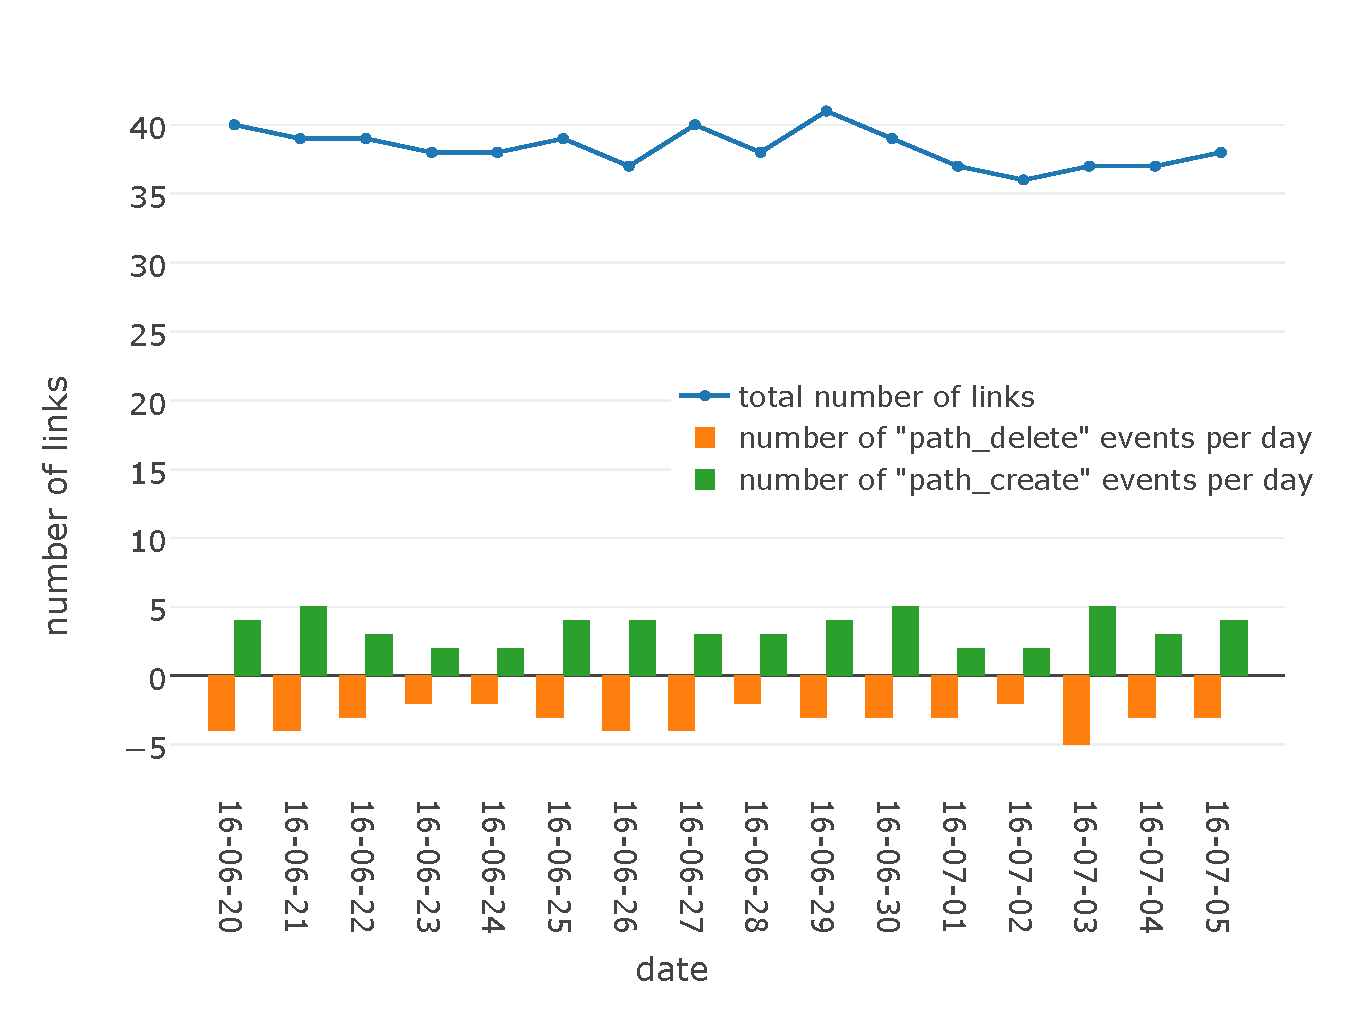
\includegraphics[width=0.5\columnwidth]{net_churn.eps}
    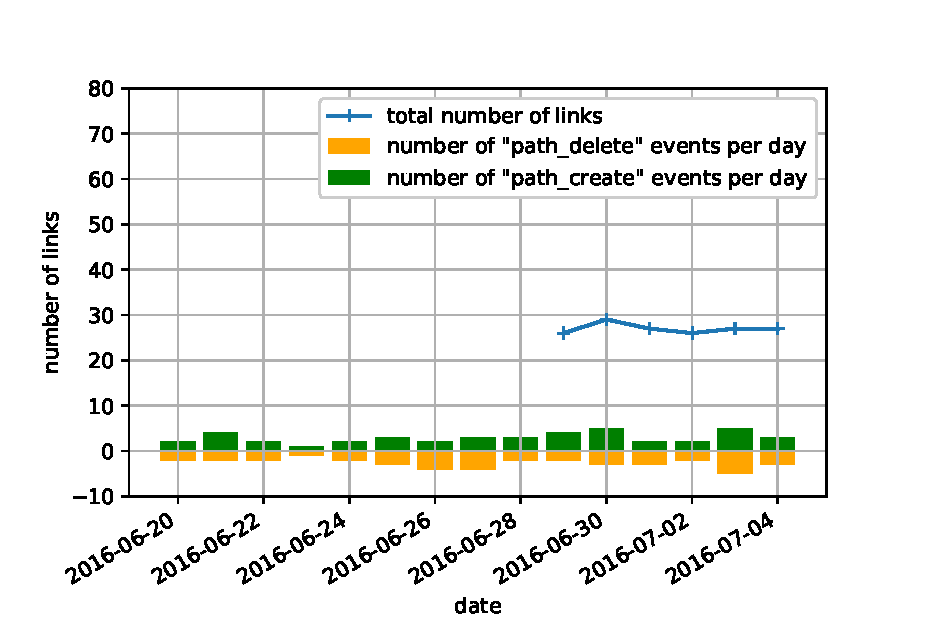
\includegraphics[width=0.5\columnwidth]{net_churn_peach.eps}
    \caption{
        Network stability: the number of \pathcreate and \pathdelete events generated per day over a 16-day period.
        The top portion shows the total number of links.
    }
    \label{fig:net_churn}
\end{figure}

% discussion

\lorem

%==============================================================================
\section{Conclusion}
\label{sec:conclusion}

% intro

\lorem

% intuitive

\lorem

% non-intuitive

\lorem

% conclusion

\lorem

%==============================================================================
%\bibliographystyle{abbrv}
%\bibliography{brun16intuitive}

\begin{thebibliography}{10}

\bibitem{std_ieee802154_2011}
{802.15.4-2011: IEEE Standard for Local and metropolitan area networks. Part
  15.4: Low-Rate Wireless Personal Area Networks (LR-WPANs)}, 5 September 2011.

\bibitem{std_ieee802154e_2012}
{802.15.4e-2012: IEEE Standard for Local and metropolitan area networks--Part
  15.4: Low-Rate Wireless Personal Area Networks (LR-WPANs) Amendment 1: MAC
  sublayer}, 16 April 2012.

\bibitem{rfc3626}
T.~H. Clausen and P.~Jacquet.
\newblock {Optimized Link State Routing Protocol (OLSR)}, October 2003.

\bibitem{smip_app_note}
Linear Technology.
\newblock {\em {SmartMesh IP Application Notes}}, 2015.

\newpage

\bibitem{saunders07antennas}
S.~R. Saunders and A.~Arag\'on-Zavala.
\newblock {\em {Antennas and Propagation for Wireless Communication Systems}}.
\newblock Wiley-Blackwell, 2nd edition, 2007.

\bibitem{srinivasan08beta}
K.~Srinivasan, M.~A. Kazandjieva, S.~Agarwal, and P.~Levis.
\newblock {The $\beta$-factor: Measuring Wireless Link Burstiness}.
\newblock In {\em Conference on Embedded Network Sensor Systems (SenSys)},
  pages 29--42, Raleigh, NC, USA, 2008. ACM.

\bibitem{watteyne16peach}
T.~Watteyne, A.~L. Diedrichs, K.~Brun-Laguna, J.~E. Chaar, D.~Dujovne, J.~C.
  Taffernaberry, and G.~Mercado.
\newblock {PEACH: Predicting Frost Events in Peach Orchards Using IoT
  Technology}.
\newblock {\em {EAI Endorsed Transactions on the Internet of Things}}, June
  2016.

\bibitem{watteyne10mitigating}
T.~Watteyne, S.~Lanzisera, A.~Mehta, and K.~S. Pister.
\newblock {Mitigating Multipath Fading through Channel Hopping in Wireless
  Sensor Networks}.
\newblock In {\em IEEE International Conference on Communications (ICC)}, pages
  1--5, Cape Town, South Africa, 23-27 May 2010. IEEE.

\bibitem{watteyne09reliability}
T.~Watteyne, A.~Mehta, and K.~Pister.
\newblock {Reliability Through Frequency Diversity: Why Channel Hopping Makes
  Sense}.
\newblock In {\em International Symposium on Performance Evaluation of Wireless
  Ad Hoc, Sensor, and Ubiquitous Networks (PE-WASUN)}, pages 116--123,
  Tenerife, Canary Islands, Spain, 26-30 October 2009. ACM.

\bibitem{watteyne15industrial}
T.~Watteyne, J.~Weiss, L.~Doherty, and J.~Simon.
\newblock {Industrial IEEE802.15.4e Networks: Performance and Trade-offs}.
\newblock In {\em International Conference on Communications (ICC), Internet of
  Things Symposium}, London, UK, 8-12 June 2015. IEEE.

\bibitem{zats10wireless}
S.~Zats.
\newblock {Wireless Sensor Networks Scaling and Deployment in Industrial
  Automation}.
\newblock Master's thesis, University of California, Berkeley, 13 May 2010.

\end{thebibliography}

\end{document}
